\documentclass[11pt]{NSF}
\sloppy

\usepackage{latexsym}
\usepackage{graphicx}
\usepackage{draftcopy}
\usepackage{longtable}
\usepackage{hyperref}

% some definitions
 
% begin equation, itemize, etc.

\def\be{\begin{equation}}
\def\ee{\end{equation}}
\def\bi{\begin{itemize}}
\def\ei{\end{itemize}}
\def\ben{\begin{enumerate}}
\def\een{\end{enumerate}}
\def\i{\item{}}

%%%%%%%%%%%%%%%%%%%%%%%%%%%%%%%%%%%%%%%%%%%%%%%%%%%%%%%%%%%%%%
            
\begin{document}

\section{10. Frequency Response of a Stringed Instrument}

PURPOSE AND BACKGROUND

We study the frequency response of a violin when white noise or a
swept-sine excitation is applied to the bridge, or when the 
instrument is tapped at the front and back. 
Such measurements give information on the quality of an
instrument. We also simulate the resonances of the instrument with
so-called Chladni figures on a metal plate that is shaped like a
violin body.


\subsection{Theory and Experiment}

A violin is played by bowing or plucking its strings. The string
vibrations are transferred to a bridge mounted on the top plate, and
from there to the sound post placed under pressure between the top
plate and back plate of the violin body. All this couples the string
vibrations to the instrument. As a result, the violin body resonates
over a rather wide range of frequencies. The cavity of the violin acts as a
Helmholtz resonator. The wood and the air of the cavity resonate to
create the characteristic rich tone of a violin. The quality of the
sound is affected by the materials, the way the wood is shaped, the
glue for joining the components, the varnish, and the skills of the
instrument maker.

\subsubsection*{Questions}
\ben
\item
The four strings of a violin are tuned in musical fifths to the
notes G3, D4, A4, and E5. 
The lowest note on a violin is G3 and the highest is C7 
(with C7 played on the E5 string). 
What are the values of these lowest and highest frequencies?

\een

\subsection{Chladni Figures}

We use a so-called {\em Chladni plate} to simulate the vibrational patterns
of the violin body. The Chladni plate is made of sheet metal and
shaped in the form of the violin back plate. This is a very rough
approximation of a violin body, where in reality wood is used and the
plates are curved. Nonetheless, we produce resonance patterns with
some resemblance to a real violin.

To produce the vibrational patterns of the Chladni plate, we place 
it horizontally on a vibrator that is driven by a frequency generator.
We then sprinkle some sand evenly on top of the plate.
The frequency of the vibrator is slowly increased until we see clear 
vibrational patterns of the jumping sand particles on the plate. 
The resonances start at frequencies well below G3 of a real violin. 
The sand jumps around and forms patterns. The places where the
sand collects are the vibrational nodes with minimum movement of the
plate. (This is a 2-dimensional analogue of the 1-dimensional nodes of
a vibrating string.) The places where no sand is left are the
anti-nodes where the Chladni plate vibrates the most. The sand moves
away from these anti-nodal regions towards the nodal areas. 
One can produce many beautiful and strange looking patterns by
adjusting the frequency. 
Figure~\ref{f:1} shows an example of a Chladni figure having a
resonance frequency of 428~Hz.
%
\begin{figure}[hbtp]
\begin{center}
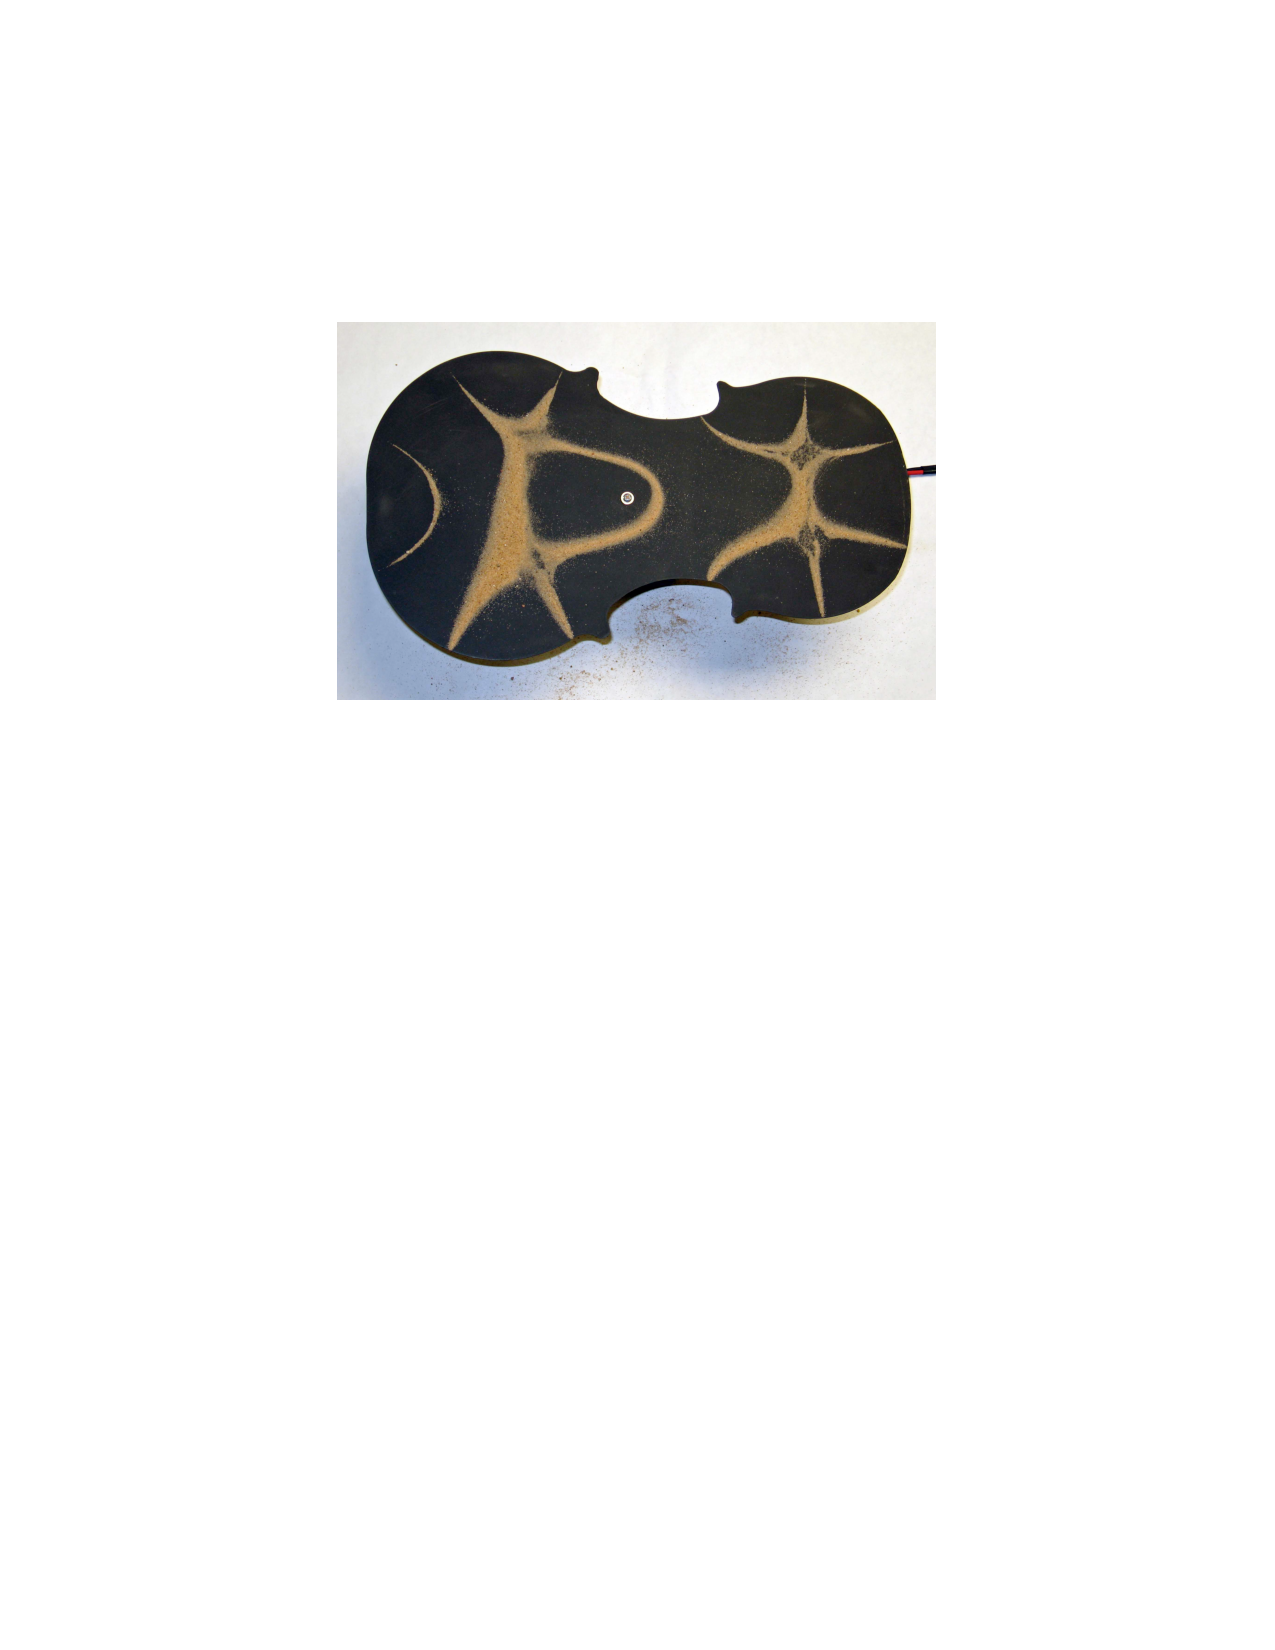
\includegraphics[width=.6\textwidth]{fig10_1}
\caption{
A Chladni figure from a metal sheet simulating the back plate of a
violin.
The resonance frequency for this pattern is 428~Hz.}
\label{f:1}
\end{center}
\end{figure}
%
Figure~\ref{f:2} shows Chladni figures for the first twelve 
resonant frequencies.
%
\begin{figure}[hbtp]
\begin{center}
\includegraphics[width=0.9\textwidth]{fig10_2}
\caption{The first 12 resonance patterns (Chladni figures) in the sand
of a vibrating metal plate. The relationship between the resonance
frequency and the resonance number is nearly linear. The photographs
show the Chladni figures for each resonance.}
\label{f:2}
\end{center}
\end{figure}
%

Our Chladni figures are not really the vibrational modes of a violin.
However, the wooden plates of a violin do show some qualitatively
similar patterns. 
The plates of a good violin exhibit one or two major wood resonances 
and air resonances in the volume of the body. 
The cavity of the body acts as a Helmholtz resonator.

\subsubsection*{Questions}
\ben
\item 
From Figure~\ref{f:2} are the resonant frequencies of the Chladni
figures harmonically related to one another?

\item 
How does the complexity of the Chladni figures change as the frequency increases?
\een

An interesting effect is seen when the resonance frequencies of the
Chladni plate are plotted versus the resonance number $N$. The first
visible resonance ($N = 1$) seen in the sand occurs at about 
$f = 100 ~{\rm Hz}$.
When the excitation frequency is increased slowly on the frequency
generator, the first 12 resonances are found to be in the range 100 to
800~Hz. Plotting these frequencies as a function of resonance number
$N$ reveals a nearly linear relationship, as seen in Figure~\ref{f:2}. 

\subsection{Response Curve of a Violin}

The study of the vibrational modes of the violin is much more
difficult than the simulation of its wood resonances with Chladni
figures. The wood has two major resonances that greatly affect the
tone and quality of a violin. Lower tones may be reinforced by a wood
resonance called wood prime resonance W’, see Figure~\ref{f:3}. 
%
\begin{figure}[hbtp]
\begin{center}
\includegraphics[width=.6\textwidth]{fig10_3}
\caption{Response curves for (a) good Stradivarius violin, (b)
“poorer” Guarneri violin. Only the Stradivarius clearly shows the wood
prime resonance W’ (left dark dot) and the wood resonance W (right
dark dot). Both violins show the air resonance (open circle). (From C.
Hutchins “The Physics of Music”, Scientific American, 1962.)}
\label{f:3}
\end{center}
\end{figure}
%
On a good
violin, the lower notes are given a boost by the W’ resonance that
contributes to a rich deep tone. An additional wood resonance W may
boost the higher frequencies. If a note is played near the frequency
regions of the wood resonances, the violin becomes louder in
intensity. Consequently, any higher harmonics that fall within these
regions increase in intensity as well, adding to the tone quality or
timbre of the instrument. The air resonance in the cavity of the
violin body (Helmholtz resonator) also increases the intensity and
quality of the sound. This resonance is determined by the volume and
shape of the violin, including the f-holes. The air resonance from
Stradivarius and Guarneri violins is shown in Figure~\ref{f:3} by the open
circle. It is seen that only the Stradivarius clearly exhibits the
wood resonances W and W’, and thus is superior to the Guarneri. (A
Guarneri generally is an excellent violin, too!)

To measure a frequency response curve for the violin, we drive the
mechanical vibrator using a stereo receiver, which is controlled by 
the FEaT software in the Mac mini, see Figure~\ref{f:4}.
%
\begin{figure}[hbtp]
\begin{center}
\includegraphics[width=.5\textwidth]{fig10_4}
\caption{Violin setup for acquiring the response curve with the FEaT
software. A microphone and a piezoelectric transducer can be used for
signal acquisition. Measurements can also be taken by moving the two
sensors to the front.}
\label{f:4}
\end{center}
\end{figure}
%
The  vibrator is connected to the bridge of the violin with a clip. 
The bridge directs
the vibration of the violin strings to the sound post in the cavity
and thus to the violin as a whole. Photographs of the violin setup are
shown in Figure~\ref{f:5}. The violin bridge rocks right and left, not
straight up and down. Therefore, the coupling from the vibrator must
be off-center in order to produce a good sound; see the clip mounting
in Figure~\ref{f:5}.
%
\begin{figure}[hbtp]
\begin{center}
\includegraphics[width=.9\textwidth]{fig10_5}
\caption{Mounting of the violin for recording the response from the
back plate (left) and front plate (right). 
The driving rod of the vibrator is fastened off-center to
the bridge of the violin with a clip. Note the microphone positions in
both pictures. (A piezoelectric transducer can be taped to the back
(or front) to complement the microphone measurements.)}
\label{f:5}
\end{center}
\end{figure}
%


The piezoelectric transducer for sensing the plate vibrations can be
taped to the back or front plate.
Similarly, the microphone can be placed near the front or
back plate. 
For the front plate, the microphone should be positioned close to 
the f-holes of the violin. 
Using white noise or a swept-sine excitation for the vibrator, 
we are able to produce frequency response curves measured 
near the front and back plates of the violin, like those 
shown in Figure~\ref{f:6}.
Several resonances are visible in the figure.
%
\begin{figure}[hbtp]
\begin{center}
\includegraphics[width=.7\textwidth]{fig10_6}
\caption{Response curves of a violin on a linear amplitude scale,
excited with white noise by a vibrator on the bridge of the violin.
Red curve: Microphone near front plate. Black curve: Microphone near
back plate. (Ordinate scale: The red resonance at 280 Hz is about 500
mV.)}
\label{f:6}
\end{center}
\end{figure}
%

\subsubsection*{Questions}
\ben
\item
Comment on the main similarities and differences of the two frequency
response curves in Figure~\ref{f:6}.

\item
Can you definitively say which peak in Figure~\ref{f:6} is the air
resonance? How can you be sure? What is the frequency of the air
resonance?

\een

\subsection{Alternative Excitation of the Violin with Tap Tones}

An easy way for exciting the violin vibrations is tapping the back
plate. The result is not the same as exciting the front plate with a
vibrator. But it offers additional information. Tapping the back plate
of the body excites the resonances similar to applying a noise
spectrum. Figure~\ref{f:7} shows a response curve obtained this way.
%
\begin{figure}[hbtp]
\begin{center}
\includegraphics[width=.7\textwidth]{fig10_7}
\caption{Violin response from tapping the back plate, with the microphone near
the front plate. The pronounced peak near 280~Hz is most likely from
the air resonance inside the violin body.}
\label{f:7}
\end{center}
\end{figure}
%

\subsubsection*{Questions}
\ben
\item
Look at the response curves in Figure~\ref{f:6} and Figure~\ref{f:7}. 
Can you
detect the air resonance and wood resonances W’ and W? Hint: See
Figure~\ref{f:3} for the approximate locations of the resonances from two
excellent violins. 
(For reference, the frequencies of the open strings of the violin
are ${\rm G3} = 196.00~{\rm Hz}$, ${\rm D4} = 293.66~{\rm Hz}$, 
${\rm A4} = 440.00~{\rm Hz}$, ${\rm E5} = 659.26~{\rm Hz}$.)

\item
Compare Figure~\ref{f:7} for our violin with the response curves of the two
violins in Figure~\ref{f:3}. 
How would you rate the quality of our violin?

\item
Suppose a violinist bowed the four open strings with equal pressure. 
Which string(s) would you expect to sound louder than others, based on
the response curves shown in Figures~\ref{f:6} and \ref{f:7}?
\een

\end{document}

